\documentclass[tikz,border=3pt]{standalone}
\usepackage[utf8]{inputenc}
\usepackage[T1]{fontenc}
\usepackage{lmodern}
\renewcommand{\familydefault}{\sfdefault}
\usepackage{sansmath}\sansmath
\usepackage{pgfplots}\pgfplotsset{compat=1.18,/pgf/number format/use comma,/pgf/number format/1000 sep={.}}
\usetikzlibrary{arrows.meta,calc,positioning,decorations.pathmorphing,patterns}
% paleta del sitio
\definecolor{nar}{HTML}{E8680C}\definecolor{narc}{HTML}{FFB35C}\definecolor{hielo}{HTML}{FFF3E8}
\definecolor{tinta}{HTML}{1D1D1F}\definecolor{gris}{HTML}{6E6E73}\definecolor{lila}{HTML}{7C5CF0}
\definecolor{azul}{HTML}{2F6FD6}\definecolor{menta}{HTML}{17A673}\definecolor{coral}{HTML}{E8342A}
% organelos
\tikzset{
 mito/.pic={
  \draw[nar!75!black,fill=narc!55,line width=0.6pt] (0,0) ellipse (0.5 and 0.24);
  \begin{scope}\clip (0,0) ellipse (0.42 and 0.17);
   \fill[hielo] (-0.5,-0.3) rectangle (0.5,0.3);
   \foreach \x/\s in {-0.3/1,-0.15/-1,0/1,0.15/-1,0.3/1} \draw[nar!75!black,line width=0.7pt] (\x,-0.2*\s) -- (\x,0.07*\s);
  \end{scope}
  \draw[nar!75!black,line width=0.6pt] (0,0) ellipse (0.42 and 0.17);
 },
 cloro/.pic={
  \draw[menta!55!black,fill=menta!30,line width=0.6pt] (0,0) ellipse (0.55 and 0.27);
  \draw[menta!55!black,line width=0.4pt] (0,0) ellipse (0.49 and 0.22);
  \draw[menta!55!black,line width=0.6pt] (-0.36,0)--(0.36,0);
  \foreach \x in {-0.26,0,0.26} \foreach \y in {-0.105,-0.035,0.035,0.105} \fill[menta!55!black] (\x-0.07,\y-0.025) rectangle (\x+0.07,\y+0.025);
 },
 golgi/.pic={
  \foreach \i in {0,1,2,3} {
   \draw[lila!75!black,line width=4.2pt,line cap=round] (0.17*\i,-0.55+0.07*\i) to[bend right=40] (0.17*\i,0.55-0.07*\i);
   \draw[lila!22,line width=2.6pt,line cap=round] (0.17*\i,-0.55+0.07*\i) to[bend right=40] (0.17*\i,0.55-0.07*\i);
  }
  \foreach \p in {(0.88,0.38),(0.95,-0.02),(0.84,-0.4),(-0.3,0.3),(-0.26,-0.32)} \draw[lila!75!black,fill=lila!22,line width=0.5pt] \p circle (0.07);
 },
 rer/.pic={
  \foreach \y in {0,0.3,0.6} {
   \draw[azul!70!black,line width=4pt,line cap=round] plot[domain=0:1.6,samples=40,smooth] (\x,{\y+0.06*sin(\x*450)});
   \draw[azul!15,line width=2.4pt,line cap=round] plot[domain=0:1.6,samples=40,smooth] (\x,{\y+0.06*sin(\x*450)});
   \foreach \t in {0.05,0.2,...,1.56} { \fill[tinta] (\t,{\y+0.06*sin(\t*450)+0.1}) circle (0.028); \fill[tinta] (\t+0.07,{\y+0.06*sin((\t+0.07)*450)-0.1}) circle (0.028);}
  }
 },
 rel/.pic={
  \foreach \y/\f in {0/0,0.32/90,0.64/200} {
   \draw[azul!55!black,line width=4pt,line cap=round] plot[domain=0:1.3,samples=40,smooth] (\x,{\y+0.09*sin(\x*360+\f)});
   \draw[azul!8,line width=2.4pt,line cap=round] plot[domain=0:1.3,samples=40,smooth] (\x,{\y+0.09*sin(\x*360+\f)});
  }
 },
 lis/.pic={\draw[coral!80!black,fill=coral!22,line width=0.6pt] (0,0) circle (0.2); \foreach \p in {(-0.07,0.05),(0.06,0.08),(0.02,-0.08),(-0.07,-0.07),(0.1,-0.01)} \fill[coral!80!black] \p circle (0.022);},
 perox/.pic={\draw[gris!90!black,fill=gris!12,line width=0.6pt] (0,0) circle (0.18); \fill[gris!80,rotate=45] (-0.06,-0.06) rectangle (0.06,0.06);},
 centri/.pic={\draw[gris!90!black,fill=gris!35,line width=0.5pt] (-0.07,-0.22) rectangle (0.07,0.22); \draw[gris!90!black,fill=gris!35,line width=0.5pt] (0.14,-0.07) rectangle (0.58,0.07);},
 vesi/.pic={\draw[lila!75!black,fill=lila!22,line width=0.5pt] (0,0) circle (0.09);},
 gran/.pic={\draw[nar!80!black,fill=nar!70,line width=0.4pt] (0,0) circle (0.11);},
}
\newcommand{\ribo}[2]{\fill[tinta] (#1,#2) circle (0.032);}
\newcommand{\nucleo}[3]{% x y r
 \draw[lila!75!black,fill=lila!10,line width=0.6pt] (#1,#2) circle (#3);
 \draw[lila!75!black,line width=0.6pt] (#1,#2) circle (#3-0.07);
 \foreach \a in {15,75,135,195,255,315} \fill[lila!10] ($(#1,#2)+(\a:#3-0.035)$) circle (0.045);
 \fill[lila!55] (#1+0.2*#3,#2+0.15*#3) circle (0.3*#3);
 \foreach \a/\d in {200/0.55,250/0.45,320/0.6,120/0.6} \draw[lila!45,line width=0.8pt] ($(#1,#2)+(\a:\d*#3)$) ++(-0.08,0) .. controls +(0.05,0.08) and +(-0.05,-0.08) .. ++(0.16,0);
}
% rótulo: punto, extremo del texto, ancla, texto
\newcommand{\lab}[4]{\fill[tinta] (#1) circle (0.03); \draw[gris,line width=0.5pt] (#1) -- (#2) node[anchor=#3,text=tinta,inner sep=2pt,align=left,font=\small] {#4};}
% rótulo numerado: punto, posición del número, número
\newcommand{\num}[3]{\fill[tinta] (#1) circle (0.03); \draw[gris,line width=0.5pt] (#1) -- (#2) node[circle,fill=nar,text=white,inner sep=1.3pt,font=\footnotesize\bfseries] {#3};}
\begin{document}
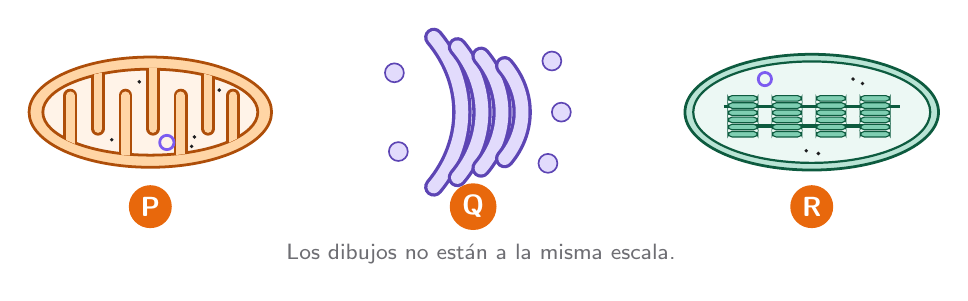
\begin{tikzpicture}[font=\small]

\begin{scope}[scale=0.7]
\draw[nar!75!black,fill=narc!55,line width=1pt] (0,0) ellipse (2.2 and 1.0);
\draw[nar!75!black,fill=hielo,line width=1pt] (0,0) ellipse (1.95 and 0.78);
\begin{scope}\clip (0,0) ellipse (1.97 and 0.8);
 \foreach \x/\s in {-1.45/1,-0.95/-1,-0.45/1,0.05/-1,0.55/1,1.05/-1,1.5/1} {
   \draw[nar!75!black,line width=5pt,line cap=round] (\x,-1.0*\s) -- (\x,0.3*\s);
   \draw[narc!55,line width=3pt,line cap=round] (\x,-1.1*\s) -- (\x,0.3*\s);
 }
\end{scope}
\draw[lila,line width=1pt] (0.3,-0.55) circle (0.13);
\foreach \p in {(0.8,-0.45),(0.75,-0.62),(-0.2,0.55),(-0.7,-0.5),(1.25,0.4)} \fill[tinta] \p circle (0.035);
\end{scope}
\node[circle,fill=nar,text=white,font=\bfseries,inner sep=2pt] at (0,-1.2) {P};
\begin{scope}[xshift=3.6cm]
\foreach \i in {0,1,2,3} {
 \draw[lila!75!black,line width=7pt,line cap=round] (0.3*\i,-0.95+0.12*\i) to[bend right=40] (0.3*\i,0.95-0.12*\i);
 \draw[lila!22,line width=4.6pt,line cap=round] (0.3*\i,-0.95+0.12*\i) to[bend right=40] (0.3*\i,0.95-0.12*\i);
}
\foreach \p in {(1.5,0.65),(1.62,0),(1.45,-0.65),(-0.5,0.5),(-0.45,-0.5)} \draw[lila!75!black,fill=lila!22,line width=0.6pt] \p circle (0.12);
\end{scope}
\node[circle,fill=nar,text=white,font=\bfseries,inner sep=2pt] at (4.1,-1.2) {Q};
\begin{scope}[xshift=8.4cm,scale=0.7]
\draw[menta!55!black,fill=menta!30,line width=1pt] (0,0) ellipse (2.3 and 1.05);
\draw[menta!55!black,fill=menta!8,line width=0.8pt] (0,0) ellipse (2.15 and 0.92);
\draw[menta!55!black,line width=1.2pt] (-1.6,0.1) -- (1.6,0.1) (-1.3,-0.25) -- (1.4,-0.25);
\foreach \x in {-1.25,-0.45,0.35,1.15} \foreach \k in {0,...,5} \draw[menta!55!black,fill=menta!55,line width=0.4pt,rounded corners=1.5pt] (\x-0.27,-0.45+0.13*\k) rectangle (\x+0.27,-0.45+0.13*\k+0.1);
\draw[lila,line width=1pt] (-0.85,0.6) circle (0.12);
\foreach \p in {(0.75,0.6),(0.92,0.52),(-0.1,-0.7),(0.12,-0.75)} \fill[tinta] \p circle (0.035);
\end{scope}
\node[circle,fill=nar,text=white,font=\bfseries,inner sep=2pt] at (8.4,-1.2) {R};
\node[font=\footnotesize,text=gris] at (4.2,-1.8) {Los dibujos no están a la misma escala.};

\end{tikzpicture}
\end{document}
